\documentclass[10pt,dvipdfmx]{beamer}
\usepackage{pgfpages}
\usepackage{graphicx}
\DeclareGraphicsExtensions{.eps}

\graphicspath{{out/tex/svg/}}

\usepackage{listings}
\usepackage{fancybox}
\usepackage{hyperref}

%%%%%%%%%%%%%%%%%%%%%%%%%%%
%%% themes
%%%%%%%%%%%%%%%%%%%%%%%%%%%
%\usetheme{Szeged} 
\usetheme{default} 
%% no navigation bar
% default boxes Bergen Boadilla Madrid Pittsburgh Rochester
%% tree-like navigation bar
% Antibes JuanLesPins Montpellier
%% toc sidebar
% Berkeley PaloAlto Goettingen Marburg Hannover Berlin Ilmenau Dresden Darmstadt Frankfurt Singapore Szeged
%% Section and Subsection Tables
% Copenhagen Luebeck Malmoe Warsaw

%%%%%%%%%%%%%%%%%%%%%%%%%%%
%%% innerthemes
%%%%%%%%%%%%%%%%%%%%%%%%%%%
% \useinnertheme{circles}	% default circles rectangles rounded inmargin

%%%%%%%%%%%%%%%%%%%%%%%%%%%
%%% outerthemes
%%%%%%%%%%%%%%%%%%%%%%%%%%%
% outertheme
% \useoutertheme{default}	% default infolines miniframes smoothbars sidebar sprit shadow tree smoothtree


%%%%%%%%%%%%%%%%%%%%%%%%%%%
%%% colorthemes
%%%%%%%%%%%%%%%%%%%%%%%%%%%
\usecolortheme{seahorse}
%% special purpose
% default structure sidebartab 
%% complete 
% albatross beetle crane dove fly seagull 
%% inner
% lily orchid rose
%% outer
% whale seahorse dolphin

%%%%%%%%%%%%%%%%%%%%%%%%%%%
%%% fontthemes
%%%%%%%%%%%%%%%%%%%%%%%%%%%
\usefonttheme{serif}  
% default professionalfonts serif structurebold structureitalicserif structuresmallcapsserif

%%%%%%%%%%%%%%%%%%%%%%%%%%%
%%% generally useful beamer settings
%%%%%%%%%%%%%%%%%%%%%%%%%%%
% 
\AtBeginDvi{\special{pdf:tounicode EUC-UCS2}}
% do not show navigation
\setbeamertemplate{navigation symbols}{}
% show page numbers
\setbeamertemplate{footline}[frame number]


%%%%%%%%%%%%%%%%%%%%%%%%%%%
%%% define some colors for convenience
%%%%%%%%%%%%%%%%%%%%%%%%%%%

\newcommand{\mido}[1]{{\color{green}#1}}
\newcommand{\mura}[1]{{\color{purple}#1}}
\newcommand{\ore}[1]{{\color{orange}#1}}
\newcommand{\ao}[1]{{\color{blue}#1}}
\newcommand{\aka}[1]{{\color{red}#1}}

\setbeamercolor{ex}{bg=cyan!20!white}

%%%%%%%%%%%%%%%%%%%%%%%%%%%
%%% how to typset code
%%%%%%%%%%%%%%%%%%%%%%%%%%%

\lstset{language = C,
numbers = left,
numberstyle = {\tiny \emph},
numbersep = 10pt,
breaklines = true,
breakindent = 40pt,
frame = tlRB,
frameround = ffft,
framesep = 3pt,
rulesep = 1pt,
rulecolor = {\color{blue}},
rulesepcolor = {\color{blue}},
flexiblecolumns = true,
keepspaces = true,
basicstyle = \ttfamily\scriptsize,
identifierstyle = ,
commentstyle = ,
stringstyle = ,
showstringspaces = false,
tabsize = 4,
escapechar=\@,
}

\title{数学・物理をプログラミングで考える}
\institute{}
\author{田浦健次朗(金1)・山崎俊彦(金4)}
\date{}

\AtBeginSubsection[] % Do nothing for \section*
{
\begin{frame}
\frametitle{Contents}
\tableofcontents[currentsection,currentsubsection]
\end{frame}
}

\begin{document}
% \maketitle

%%%%%%%%%%%%%%%%% 
\begin{frame}[fragile]
\frametitle{数学・物理をプログラミングで考える \\
\hspace{\fill}{\small 田浦健次朗(金1)・山崎俊彦(金4)}
}

\begin{center}
\ao{\bf\large 内容: 物理・数学の問題をコンピュータ(数値計算)で解く}

\begin{itemize}
\item ホームページ: {\small \url{http://pmp.eidos.ic.i.u-tokyo.ac.jp/} (\url{http://bit.ly/1ZFu6q2})}
\item \href{https://drive.google.com/file/d/19l28PFQxVEDzwYXShu46IpKoPvgvd3z-/view?usp=sharing}{動画}
\end{itemize}

\end{center}

\begin{columns}
\begin{column}{0.5\textwidth}

\begin{figure}[htbp]
\begin{center}
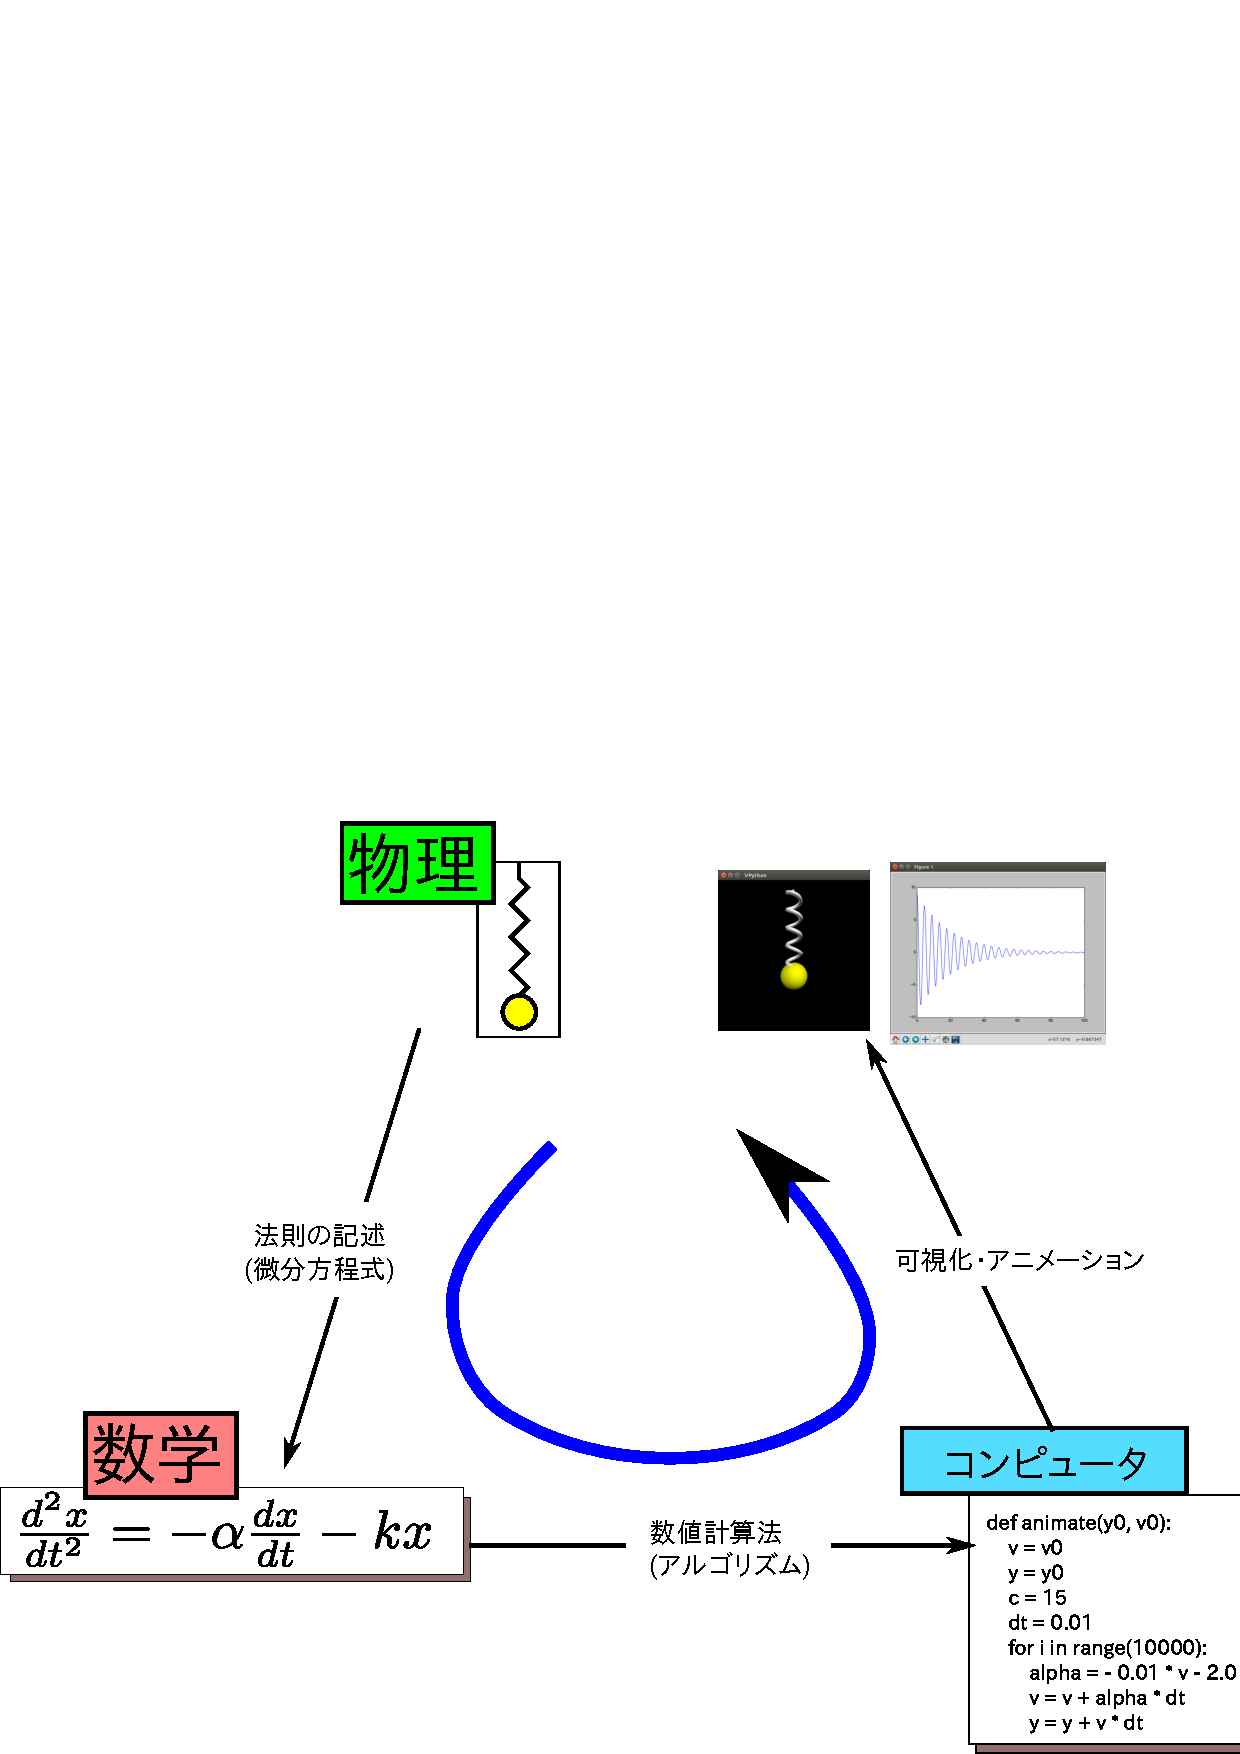
\includegraphics[width=\textwidth]{out/pdf/svg/math_phys_prog_3.pdf}
\end{center}
\end{figure}
\end{column}

\begin{column}{0.53\textwidth}

目標:
\begin{itemize}
\item 実際の問題を数値計算で解く \\
$\rightarrow$ \ao{プログラミングを学ぶ動機}
\item そのための物理や数学を学ぶ \\
$\rightarrow$ \ao{数学・物理を学ぶ動機}
\item 解決のための,\aka{自発的な勉強,試行錯誤}
\end{itemize}
\end{column}
\end{columns}

モットー:
\begin{center}
\begin{itemize}
\item 物理法則の価値・すごさを「解ける」ことで実感 \\
  {\footnotesize (シュレディンガー,ナビエストークス,解析力学,\ldots)}
\item 大学数学の価値・すごさを「解くために使う」ことで実感 \\
  {\footnotesize ($n\times n$行列, 多変数の微積分, 偏微分方程式, \ldots)}
\end{itemize}
\end{center}

\end{frame}


%%%%%%%%%%%%%%%%% 
\begin{frame}
\frametitle{身につくスキル・進行形式}
\begin{columns}
  \begin{column}{0.6\textwidth}

    スキル:
    \begin{itemize}
    \item 簡単・強力な\ao{プログラミング言語: Python}
    \item 強力な\ao{ライブラリ・パッケージ:}
      3Dアニメーション, データ可視化, 行列計算, 最大最小化, 方程式, \ldots
    \end{itemize}

    形式:
    \begin{itemize}
    \item 数人のグループで, 作戦会議と作業
    \item 進捗共有・議論のためのミニ発表(数件/週)
    \item 最終回発表
    \item 進行(目安) 
      
      {\scriptsize \begin{tabular}{|l|l|}\hline
          1-2  & ガイダンス, 共通授業 \\\hline
          3    & イントロ, Python練習 \\\hline
          4-5  & Python練習, 最終課題予告 \\\hline
          6-12 & Python練習, 最終課題に向けた議論, 作業(プログラミング) \\\hline
          13   & 発表会 \\\hline
        \end{tabular}}
    \end{itemize}

  \end{column}

  \begin{column}{0.4\textwidth}
    \begin{center}
    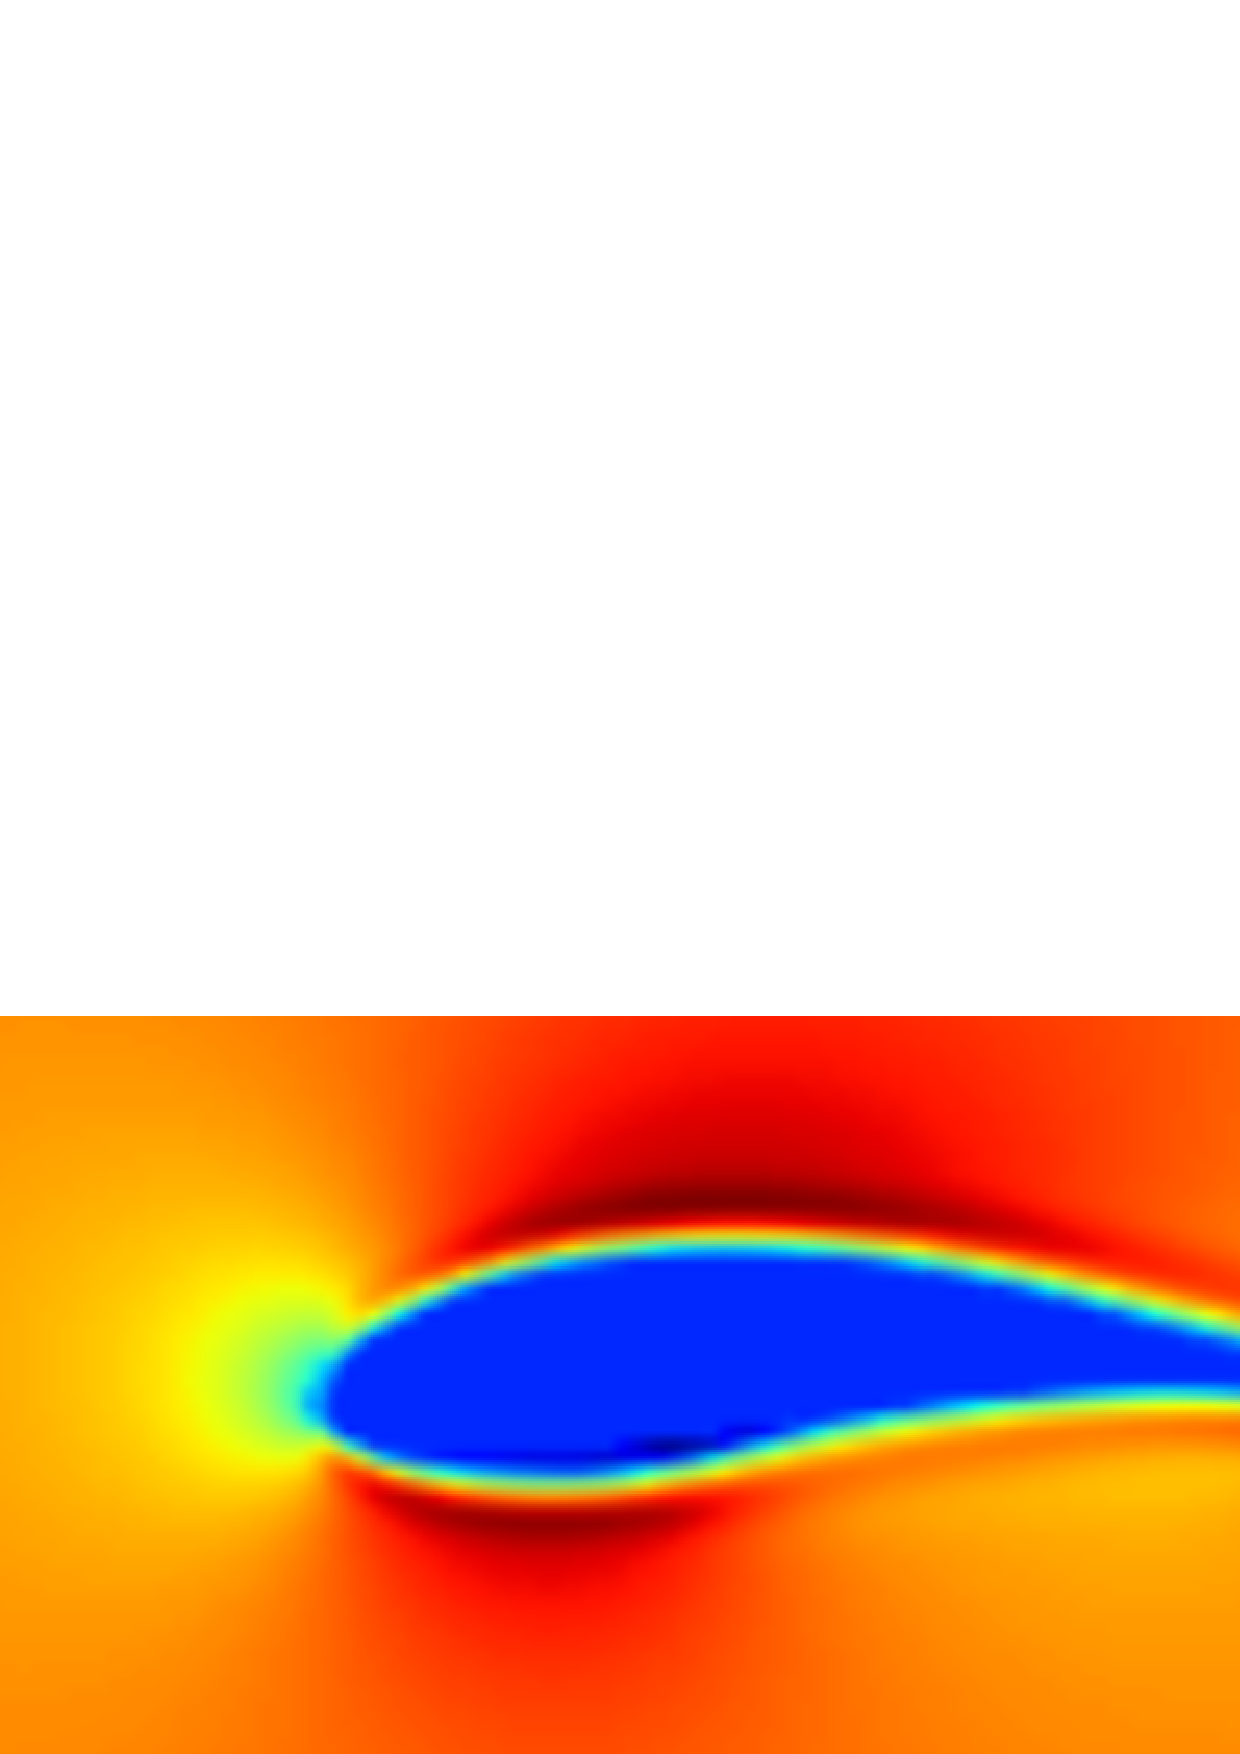
\includegraphics[width=0.9\textwidth]{out/pdf/img/wing2.pdf}

    \begin{minipage}[t]{0.3\textwidth}
      \vskip-2cm
      \includegraphics[width=\textwidth]{out/pdf/img/surface3d_demo_hires.pdf} \\
      \includegraphics[width=\textwidth]{out/pdf/img/image_interp_00_hires.pdf}
    \end{minipage}
    \begin{minipage}[t]{0.5\textwidth}
      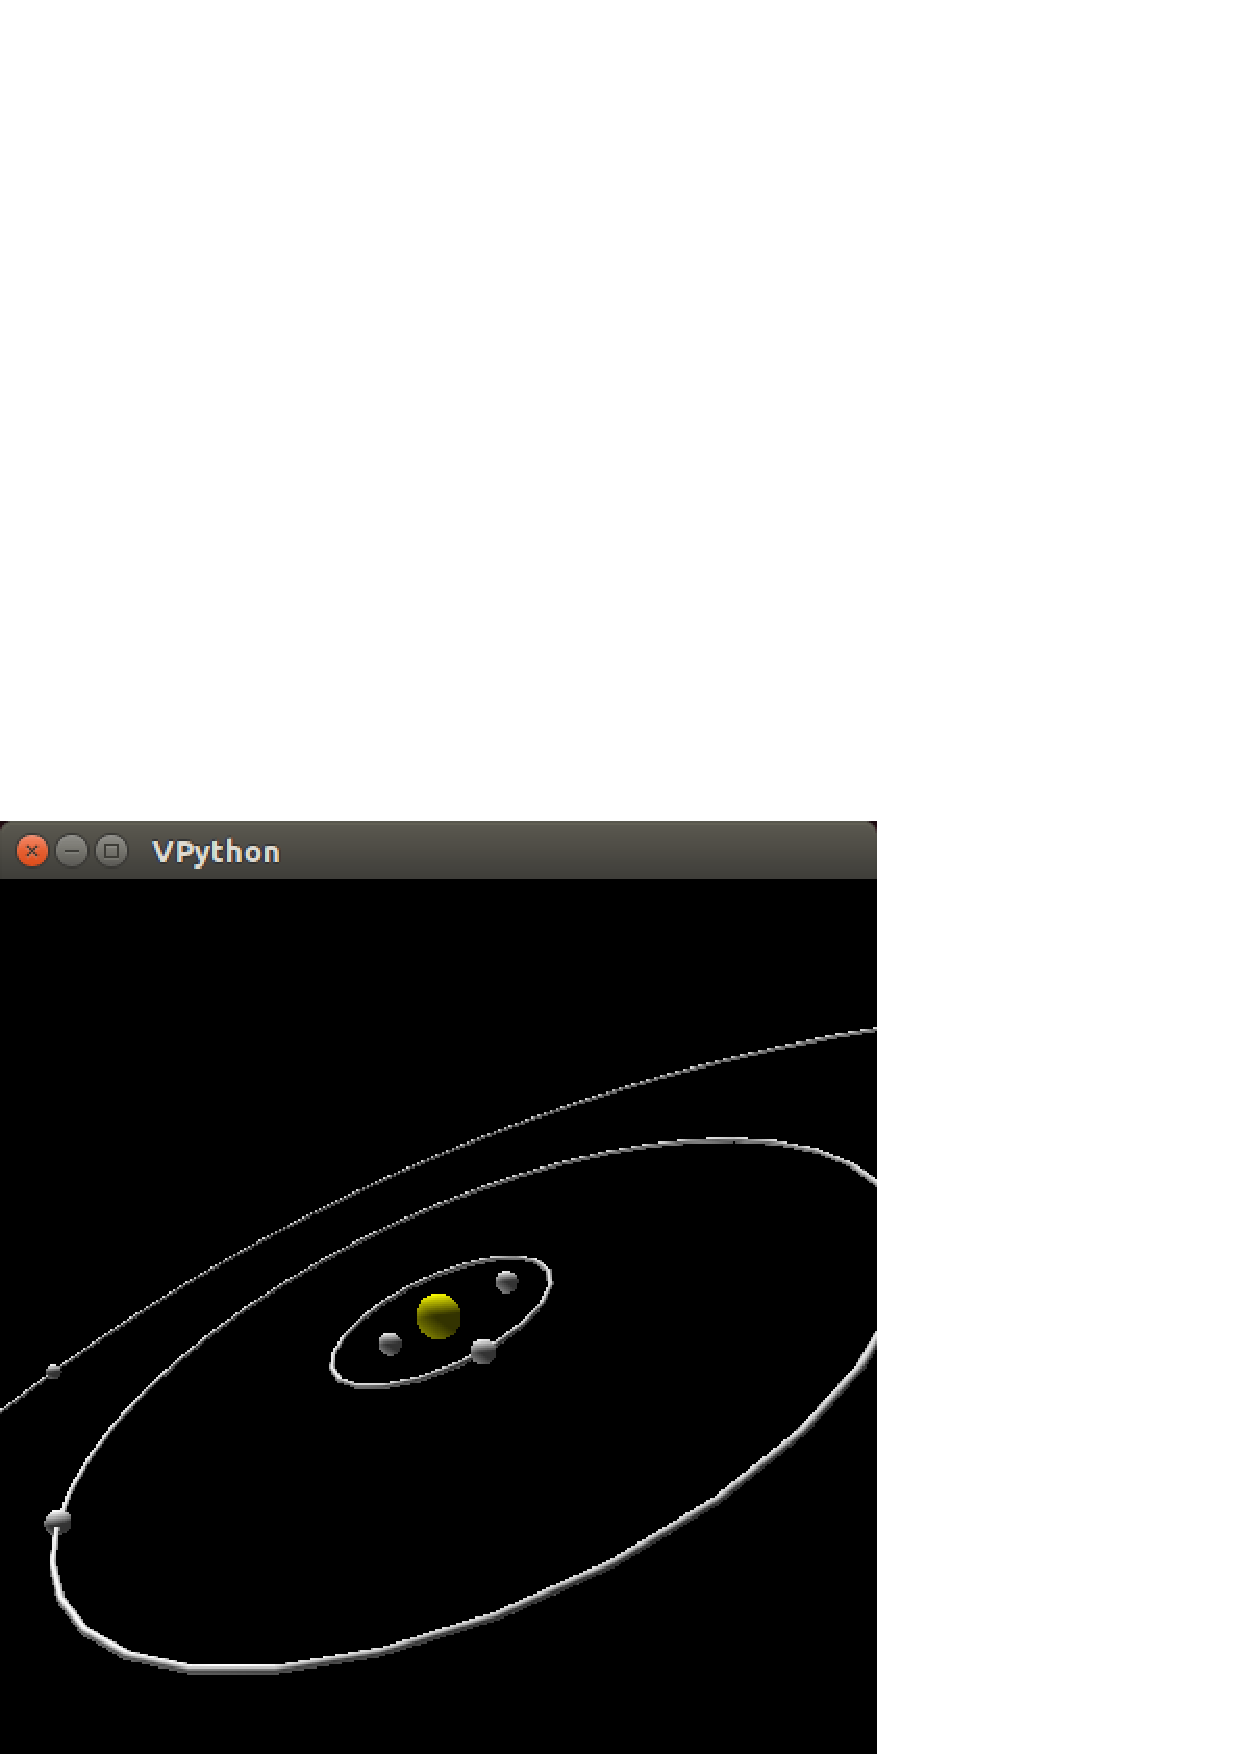
\includegraphics[width=\textwidth]{out/pdf/img/solar_system.pdf}
    \end{minipage}

  \includegraphics[width=0.45\textwidth]{out/pdf/img/snap3.pdf}
    \hspace{0.2cm}\includegraphics[width=0.45\textwidth]{out/pdf/img/snap7.pdf}

    \hspace{0.5cm}\includegraphics[width=0.8\textwidth]{out/pdf/img/snap4.pdf}

    \end{center}

  \end{column}
\end{columns}

\end{frame}

\end{document}



